\section{Обзор предметной области}
\label{sec:domain}

\subsection{Постановка задачи}
\label{sub:domain:problem_formulation}
Целью данного дипломного проекта является создание веб-сервиса, состоящего из серверной и клиентской частей с использованиям Ruby on Rails, AngularJS, Sidekiq, для получения уведомлений о новинках в музыкальной индустрии.

Для реализации данного проекта можно выделить следующие минимальные требования:

\begin{itemize}
  \item Система должна быть компонентной, то есть разделённой на отдельные модули. Это облегчает разработку, внесение изменений и тестирование.
  \item Система должна поддерживать мультиязычность для охвата большей аудитории с возможностью добавления новых языков и редактирования старых.
  \item Система должна соответствовать современным требованиям к интерфейсам быть удобной для пользователя.
  \item Система должна быть выполнена в виде SPA-приложения с использованием асинхронных запросов.
  \item Система должна быть легко масштабируема для добавления новых источников публикаций.
  \item Система должна быть имплементирована с наличием авторизации, аутентификации, разных ролей, в том числе администраторской.
\end{itemize}

Для реализации вышеописанных требований необходимо решить следующие задачи:

\begin{itemize}
  \item Изучить аналоги, присутствующие на рынке, для того, чтобы учесть ошибки и недостатки изучаемых сервисов, а также выделить сильные стороны и использовать их в разработке.
  \item Изучить предметную область, портрет целевой аудитории, чтобы лучше понимать нужды и правильно реализовать их в системе.
  \item Выбрать и изучить подходящие технологии для разработки сервиса.
  \item Создать архитектуру, которая будет удовлетворять требованиям разработки и реализовать её с использованием выбранных технологий.
\end{itemize}

\subsection{Обзор существующих аналогов}
\label{sub:domain:analogues_review}
В данном разделе будут рассмотрены приложения, которые по логике своей работы пересекаются с тематикой данной дипломной работы, а именно предоставляют пользователям возможность узнавать о новинках музыкальной индустрии. Некоторые из них является веб-сервисами, направленными на видеоконтент, другие -- на музыкальный. И те, и другие выполняют свою задачу и направлены на свою целевую аудиторию. Рассмотрим несколько из вышеописанных сервис.

\subsubsection{YouTube Just Released Music Videos}
\label{sub:domain:analogues_review:youtube}
~\newline
\indent YouTube -- видеохостинговый сервис, предоставляющий пользователям загружать свои видео, делать их некоторую обработку и получать статистику просмотров. Также на YouTube есть комментарии, кнопки “мне нравится” и “мне не нравится”. Таким образом данный сервис имеет большую вовлечённость пользователей.

Однако в данной дипломной работе рассматривается отдельный сервис, который пересекается с её тематикой -- это Just Released Music Videos. Эта площадка показывает людям последние публикации артистов. Другими словами, Just Released Music Videos демонстрирует пользователям список из только что издававшихся видео-роликов певцов, музыкантов, музыкальных коллективов. Данный сервис интегрирован в YouTube и является его частью.

Список видеороликов, представленный в Just Released Music Videos отсортирован в порядке убывания по дате публикации, то есть, чем новее видео, тем выше в этом списке оно поднимается, что логично для пользователя, который ожидает увидеть именно новинки музыкальной индустрии. Также напротив видео будет указана длительность композиции и небольшая картинка, которая является превью к видео.

У данного сервиса можно выделить следующие преимущества:

\begin{itemize}
  \item позволяет пользователю не только посмотреть музыку, но и увидеть видеоклип;
  \item позволяет пользователю видеть количество просмотров, таким образом оценивая его популярность;
  \item есть возможность включения субтитров, что является встроенной функциональностью YouTube, таким образом позволяя пользователю сразу видеть текст композиции при условии его присутствия;
\end{itemize}

Однако кроме преимуществ можно выделить следующие недостатки:

\begin{itemize}
  \item артисты, представленные в списке данного сервиса, никак не связаны с тем, что интересно пользователю, тем самым создавая лишнюю информационные данные;
  \item сервис не является самостоятельным, а интегрированным в сервис YouTube;
  \item нет возможности получения прямых уведомлений на почту;
\end{itemize}

\begin{figure}[ht]
\centering
  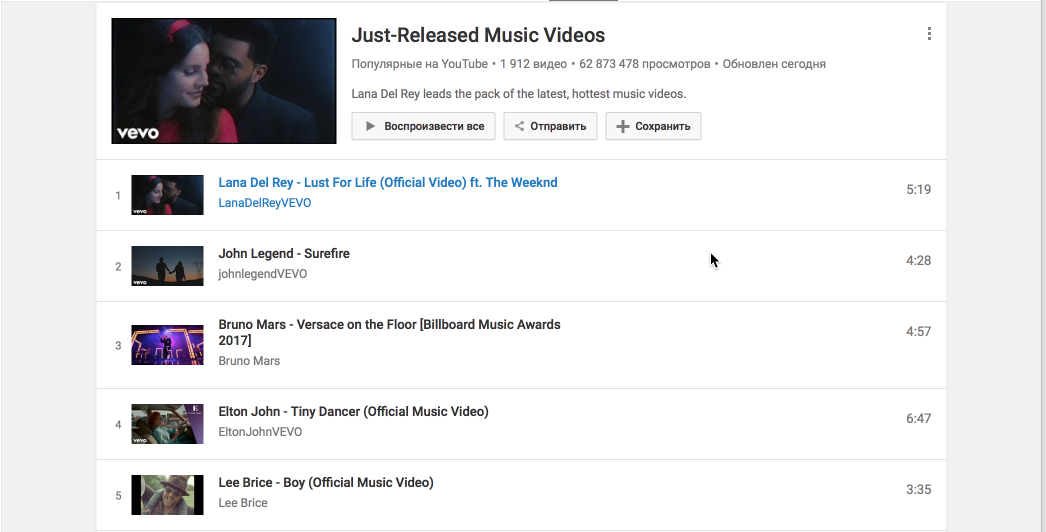
\includegraphics[scale=0.5]{youtubejustreleased.png}
  \caption{ Изображение сервиса YouTube Just Released Music Videos }
  \label{fig:domain:youtube_just_released_music_videos:picture}
\end{figure}

\subsubsection{AllMusic}
\label{sub:domain:analogues_review:allmusic}
~\newline
\indent AllMusic представляет собой американский сервис, который включает в себя крупную онлайновую музыкальную базу данных. В AllMusic представлена информация о жанрах музыки, музыкантах и коллективах, в том числе новые публикации и профессиональные рецензии. Данный сервис является обладателем огромного музыкального архива, который насчитывает около шести миллионов композиций. Также на сайте имеется возможность оценки публикаций пользователями.
AllMusic предоставляет пользователю довольно широкий спектр возможностей. Например, пользователь может подписаться на обновления, чтобы получать письма с уведомлением о новой публикации. Также есть возможность получать индивидуальные музыкальные рекомендации. Для этого необходимо заполнить артистов, которые нравятся пользователю, в поля для ввода и далее будут предложены альбомы артистов по каким-либо параметрам схожих с введёнными ранее. Я считаю, что это весьма полезная функциональность для того, чтобы найти новую музыку.
AllMusic обладает стильным, выдержанным, но, на мой взгляд, слегка загроможденным дизайном. Сервис предоставляет широкую функциональность, и по этой причине пользователю, заинтересованному лишь в получении музыкальных новинок, может мешать наличие множества разнообразных разделов. Сервис перестаёт быть сконцентрированным на одной вещи. Это, в зависимости от интересов конечного пользователя, может как оттолкнуть, так и быть интересным.

\begin{figure}[ht]
\centering
  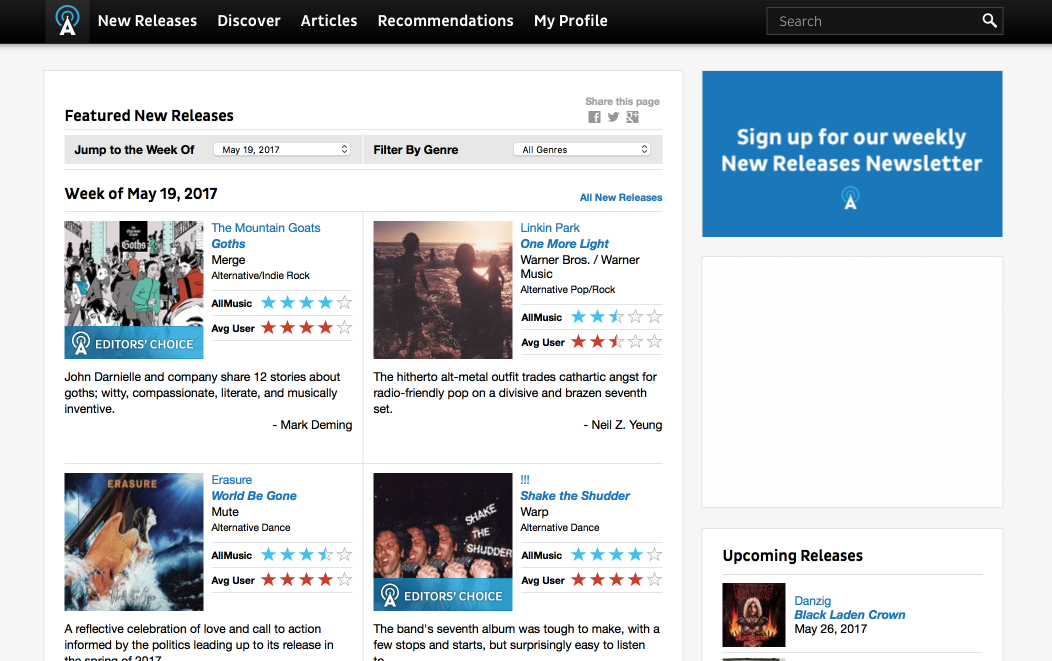
\includegraphics[scale=0.5]{allmusic.png}
  \caption{ Изображение сервиса AllMusic }
  \label{fig:domain:allmusic:picture}
\end{figure}

Преимущества AllMusic:

\begin{itemize}
  \item возможность регистрации через социальные сети;
  \item большая база данных публикаций;
  \item возможность оценивать альбомы, что позволяет пользователям судить о качестве;
  \item богатство жанров;
  \item возможность получать уведомления;
  \item наличие персональных рекомендаций;
  \item возможность прослушать отрывки композиций;
\end{itemize}

Также можно обозначить следующие недостатки:

\begin{itemize}
  \item отсутствие концентрированности на публикациях артистов, и, как следствие, массивный интерфейс;
  \item отсутствие ссылок на сервисы для приобретения альбомов;
  \item отсутствие возможности импортировать артистов с устройств/сервисов;
  \item небольшая интерактивность;
\end{itemize}

\subsubsection{Вывод}
~\label{sub:domain:analogues_review:conclusion}
\newline
\indent Учитывая результаты ознакомления с уже присутствующими аналогами сервисов для получения информации о новинках музыкальной индустрии, можно сделать вывод, что большинство подобных сервисов либо слишком усложнены, либо делают акцент не на основную потребность конечного пользователя, а именно получение уведомлений, информации о новых публикациях любимых артистов.

\subsection{Музыкальный альбом (публикация)}
\label{sub:domain:music_album}
Музыкальный альбом -- это некоторая совокупность музыкальных композиций, которые выпускаются вместе, в стандартном формате. Такие композиции должны быть доступны для произведения на популярных воспроизводящих устройствах.
Существуют классификации альбомов по нескольким признакам: по объёмы, типу записи и так далее. Некоторые из них будут рассмотрены далее.

\subsubsection{Классификация по объёму}
\label{sub:domain:music_album:volume_classification}
~\newline
\indent Музыкальные альбомы по объёму классифицируются следующим образом:
\begin{itemize}
  \item Сингл не относят к альбомам, так как состоят из одной-двух песен. Рассматривается в данной работе для большей ясности нижеприведённой информации.
  \item Стандартный альбом, или LP (от английского “Long Play”) обычно размещается на одной пластинке или же на одном компакт-диске. Время звучания насчитывает около 30-80 минут.
  \item Мини-альбом, или EP (от английского “Extended Play”) по своему размеру является промежуточным вариантом между стандартным и синглом.
  \item Двойной альбом выпускается на двух носителях информации, и время звучания такого альбома в среднем в два раза больше, чем стандартный альбом.
\end{itemize}

\subsubsection{Классификация по типам записей и композиций}
\label{sub:domain:music_album:records_type_classification}
~\newline
\indent Музыкальные альбомы по типам записей и композиций классифицируются следующим образом:
\begin{itemize}
  \item Студийный альбом -- альбом, записанный в звукозаписывающей студии.
  \item Концертный альбом -- альбом, который записывается в то время, как идёт “живое” выступление перед публикой, то есть запись концерта.
  \item “Программный” альбом -- альбом, в котором обычно содержаться только ранее не издававшиеся композиции, хотя бывают и исключения, когда в “программный” альбом включаются концертные записи.
\end{itemize}

\subsubsection{Другие типы альбомов}
\label{sub:domain:music_album:other_types_classification}
~\newline
\indent Существуют также следующие типы музыкальных публикаций:
\begin{itemize}
  \item Демо представляет собой демонстрационную запись. В ней обычно содержится “сырой” материал, который используется для ознакомления других лиц с творчеством исполнителя. Зачастую это некоторые первые записи музыкантов, которые официально не издавались.
  \item Концептуальный альбом -- это альбом, все композиции которого объединены некоторой идеей (концепцией). В таких альбомах можно усмотреть некоторый замысел в составе и порядке композиций.
  \item Промо -- альбом, который выпускается небольшим тиражом специально для бесплатного распространения с целью рекламы исполнителя.
  \item Саундтрек -- альбом, в составе которого используются композиции из одного или нескольких фильмов, компьютерных игр.
  \item Трибьют -- альбом, в котором в дань уважения и в знак почитания творчества одни исполнители переигрывают песни другого определённого исполнителя. Такие композиции называются каверами.
\end{itemize}

\subsection{API}
\label{sub:domain:api}
API(application programming interface, программный интерфейс приложения) - это совокупность процедур, функций, и классов и т.д. , которую предоставляет сервис для использования в некоторых внешних приложениях (клиентах).

API используется для того, чтобы представить функциональность программы, при этом абстрагируясь от конкретной реализации.

WebAPI -- это API, основу в котором составляют HTTP-запросы и HTTP-ответы, сконструированные по определённым принципам. API используется, как источник данных для клиентского приложения. Клиент использует HTTP-запросы с глаголами GET, POST, PATCH, DELETE и другие. При этом в теле запроса передаются необходимые параметры. Далее API принимает этот запрос, и, если необходимо, авторизирует клиент. Может использоваться ролевая авторизация, когда в системе присутствуют разные типы пользователей: администраторы, модераторы, конечные пользователи. После запрос обрабатывается, и возвращается ответ в виде XML или JSON. Ответ принимается клиентом, также обрабатывается и на основе результатов производятся необходимые действия.
